\documentclass[aspectratio=169,11pt]{beamer}

% Theme and colors
\usetheme{Madrid}
\usecolortheme{seahorse}

% Custom colors
\definecolor{primary}{RGB}{46,134,171}
\definecolor{secondary}{RGB}{162,59,114}
\definecolor{accent}{RGB}{241,143,1}

\setbeamercolor{palette primary}{bg=primary,fg=white}
\setbeamercolor{palette secondary}{bg=secondary,fg=white}
\setbeamercolor{palette tertiary}{bg=primary!80,fg=white}
\setbeamercolor{structure}{fg=primary}
\setbeamercolor{title}{fg=primary}
\setbeamercolor{frametitle}{fg=primary}
\setbeamercolor{block title}{bg=primary,fg=white}
\setbeamercolor{block body}{bg=primary!10}

% Packages
\usepackage[utf8]{inputenc}
\usepackage{amsmath,amssymb}
\usepackage{mathtools}
\usepackage{graphicx}
\usepackage{booktabs}
\usepackage{tikz}
\usetikzlibrary{shapes,arrows,positioning,calc}

% Remove navigation symbols
\setbeamertemplate{navigation symbols}{}

% Add frame numbers
\setbeamertemplate{footline}{
    \hfill\insertframenumber/\inserttotalframenumber\hspace{2mm}\vspace{2mm}
}

% Title information
\title[PCA Project]{\textbf{Principal Component Analysis}}
\subtitle{Environmental Impact of Fast Fashion Industry}
\author{ST2DA-I2 | 2025-2026}
\date{\today}
\institute{}

\begin{document}

%==============================================================================
% Title Slide
%==============================================================================
\begin{frame}
    \titlepage
\end{frame}

%==============================================================================
% Outline
%==============================================================================
\begin{frame}{Outline}
    \tableofcontents
\end{frame}

%==============================================================================
\section{Introduction}
%==============================================================================

\begin{frame}{What is PCA?}
    \begin{block}{Definition}
        Principal Component Analysis is a \textbf{linear transformation} that projects high-dimensional data onto a lower-dimensional subspace while \textbf{maximizing variance}.
    \end{block}
    
    \vspace{0.5cm}
    
    \begin{columns}
        \begin{column}{0.5\textwidth}
            \textbf{Key Properties:}
            \begin{itemize}
                \item Orthogonal transformation
                \item Variance maximization
                \item Dimensionality reduction
                \item Feature extraction
            \end{itemize}
        \end{column}
        \begin{column}{0.5\textwidth}
            \textbf{Applications:}
            \begin{itemize}
                \item Data visualization
                \item Noise reduction
                \item Feature engineering
                \item Exploratory analysis
            \end{itemize}
        \end{column}
    \end{columns}
\end{frame}

\begin{frame}{Our Dataset}
    \textbf{True Cost of Fast Fashion Dataset}
    
    \vspace{0.3cm}
    
    \begin{columns}
        \begin{column}{0.5\textwidth}
            \textbf{Overview:}
            \begin{itemize}
                \item $n = 3000$ observations
                \item $p = 25$ total attributes
                \item 15 quantitative for PCA
                \item 5 brands, 10 countries
            \end{itemize}
        \end{column}
        \begin{column}{0.5\textwidth}
            \textbf{Variable Categories:}
            \begin{itemize}
                \item \textcolor{primary}{Production}: Volume, Cycles
                \item \textcolor{secondary}{Environmental}: CO$_2$, Water, Waste
                \item \textcolor{accent}{Sustainability}: Scores, Indices
                \item \textcolor{primary!60!black}{Social}: Wages, Hours, Labor
            \end{itemize}
        \end{column}
    \end{columns}
    
    \vspace{0.5cm}
    
    \begin{alertblock}{Why PCA?}
        Variables have \textbf{different scales} (tonnes, USD, \%) $\Rightarrow$ Use \textbf{correlation-based PCA}
    \end{alertblock}
\end{frame}

\begin{frame}{Complete Dataset Attributes}
    \small
    \begin{columns}
        \begin{column}{0.48\textwidth}
            \textbf{Identifiers (3):}
            \begin{itemize}
                \item Brand, Country, Year
            \end{itemize}
            
            \vspace{0.2cm}
            \textbf{Production (2):}
            \begin{itemize}
                \item Monthly\_Production\_Tonnes
                \item Release\_Cycles\_Per\_Year
            \end{itemize}
            
            \vspace{0.2cm}
            \textbf{Environmental (3):}
            \begin{itemize}
                \item Carbon\_Emissions\_tCO2e
                \item Water\_Usage\_Million\_Litres
                \item Landfill\_Waste\_Tonnes
            \end{itemize}
            
            \vspace{0.2cm}
            \textbf{Social (3):}
            \begin{itemize}
                \item Avg\_Worker\_Wage\_USD
                \item Working\_Hours\_Per\_Week
                \item Child\_Labor\_Incidents
            \end{itemize}
        \end{column}
        \begin{column}{0.48\textwidth}
            \textbf{Economic (2):}
            \begin{itemize}
                \item Avg\_Item\_Price\_USD
                \item GDP\_Contribution\_Million\_USD
            \end{itemize}
            
            \vspace{0.2cm}
            \textbf{Consumer (4):}
            \begin{itemize}
                \item Return\_Rate\_Percent
                \item Avg\_Spend\_Per\_Customer\_USD
                \item Shopping\_Frequency\_Per\_Year
                \item Social media mentions (2)
            \end{itemize}
            
            \vspace{0.2cm}
            \textbf{Sustainability (5):}
            \begin{itemize}
                \item Env\_Cost\_Index
                \item Sustainability\_Score
                \item Transparency\_Index
                \item Compliance\_Score
                \item Ethical\_Rating
            \end{itemize}
        \end{column}
    \end{columns}
\end{frame}

%==============================================================================
\section{Mathematical Framework}
%==============================================================================

\begin{frame}{The PCA Optimization Problem}
    \begin{block}{Objective}
        Find direction $\mathbf{v}_1$ that maximizes variance of projected data:
        \begin{equation*}
            \mathbf{v}_1 = \arg\max_{\|\mathbf{v}\|=1} \text{Var}(\mathbf{Xv}) = \arg\max_{\|\mathbf{v}\|=1} \mathbf{v}^\top \mathbf{S} \mathbf{v}
        \end{equation*}
    \end{block}
    
    \vspace{0.3cm}
    
    \textbf{Lagrangian formulation:}
    \begin{equation*}
        \mathcal{L}(\mathbf{v}, \lambda) = \mathbf{v}^\top \mathbf{S} \mathbf{v} - \lambda(\mathbf{v}^\top\mathbf{v} - 1)
    \end{equation*}
    
    \textbf{First-order condition:}
    \begin{equation*}
        \frac{\partial \mathcal{L}}{\partial \mathbf{v}} = 2\mathbf{S}\mathbf{v} - 2\lambda\mathbf{v} = 0 \quad \Rightarrow \quad \boxed{\mathbf{S}\mathbf{v} = \lambda\mathbf{v}}
    \end{equation*}
    
    \begin{center}
        \textcolor{secondary}{\textbf{$\Rightarrow$ Eigenvalue problem!}}
    \end{center}
\end{frame}

\begin{frame}{Spectral Decomposition}
    \begin{theorem}[Spectral Theorem]
        For symmetric matrix $\mathbf{R} \in \mathbb{R}^{p \times p}$:
        \begin{equation*}
            \mathbf{R} = \mathbf{V}\mathbf{\Lambda}\mathbf{V}^\top = \sum_{k=1}^{p} \lambda_k \mathbf{v}_k \mathbf{v}_k^\top
        \end{equation*}
        where $\lambda_1 \geq \lambda_2 \geq \cdots \geq \lambda_p \geq 0$
    \end{theorem}
    
    \vspace{0.3cm}
    
    \textbf{Key Results:}
    \begin{itemize}
        \item Eigenvectors $\mathbf{v}_k$ are \textbf{orthonormal}: $\mathbf{V}^\top\mathbf{V} = \mathbf{I}$
        \item Eigenvalues $\lambda_k$ = \textbf{variance} of $k$-th principal component
        \item Total variance preserved: $\sum_{k=1}^{p} \lambda_k = \text{tr}(\mathbf{R}) = p$
    \end{itemize}
\end{frame}

\begin{frame}{Covariance vs. Correlation Matrix}
    \begin{columns}
        \begin{column}{0.48\textwidth}
            \begin{block}{Covariance Matrix $\mathbf{S}$}
                \begin{equation*}
                    s_{jk} = \frac{1}{n-1}\sum_{i=1}^{n}(x_{ij} - \bar{x}_j)(x_{ik} - \bar{x}_k)
                \end{equation*}
                
                \textbf{Use when:}
                \begin{itemize}
                    \item Variables have same units
                    \item Scale matters
                \end{itemize}
            \end{block}
        \end{column}
        \begin{column}{0.48\textwidth}
            \begin{block}{Correlation Matrix $\mathbf{R}$}
                \begin{equation*}
                    r_{jk} = \frac{s_{jk}}{s_j \cdot s_k}
                \end{equation*}
                
                \textbf{Use when:}
                \begin{itemize}
                    \item Variables have different units
                    \item Want equal contribution
                \end{itemize}
            \end{block}
        \end{column}
    \end{columns}
    
    \vspace{0.5cm}
    
    \begin{alertblock}{Our Choice: Correlation Matrix}
        Variables have heterogeneous units (tonnes, USD, \%, indices) $\Rightarrow$ \textbf{Standardize first!}
        \begin{equation*}
            z_{ij} = \frac{x_{ij} - \bar{x}_j}{s_j}
        \end{equation*}
    \end{alertblock}
\end{frame}

\begin{frame}{Factor Loadings \& Quality Metrics}
    \begin{block}{Factor Loadings}
        Correlation between variable $X_j$ and component $Z_k$:
        \begin{equation*}
            \ell_{jk} = v_{jk} \cdot \sqrt{\lambda_k} = \text{Corr}(X_j, Z_k)
        \end{equation*}
    \end{block}
    
    \vspace{0.3cm}
    
    \begin{columns}
        \begin{column}{0.48\textwidth}
            \textbf{Quality of Representation (cos²):}
            \begin{equation*}
                \cos^2_{j,K} = \sum_{k=1}^{K} \ell_{jk}^2
            \end{equation*}
            $\rightarrow$ How well is variable $j$ represented?
        \end{column}
        \begin{column}{0.48\textwidth}
            \textbf{Variable Contribution:}
            \begin{equation*}
                \text{CTR}_{jk} = v_{jk}^2
            \end{equation*}
            $\rightarrow$ How much does $j$ contribute to PC$_k$?
        \end{column}
    \end{columns}
\end{frame}

\begin{frame}{Component Selection Criteria}
    \textbf{How many components to retain?}
    
    \vspace{0.3cm}
    
    \begin{enumerate}
        \item \textbf{Scree Test} (Cattell, 1966):
        \begin{equation*}
            \text{Find ``elbow'' in } \{\lambda_1, \lambda_2, \ldots, \lambda_p\}
        \end{equation*}
        \textit{Rationale: Identify where eigenvalues level off}
        
        \vspace{0.3cm}
        
        \item \textbf{Variance Threshold}:
        \begin{equation*}
            \text{Retain } K \text{ s.t. } \sum_{k=1}^{K} \frac{\lambda_k}{p} \geq 0.70 \text{ or } 0.80
        \end{equation*}
        
        \vspace{0.3cm}
        
        \item \textbf{Interpretability}:
        \begin{equation*}
            \text{Components should be interpretable in domain context}
        \end{equation*}
    \end{enumerate}
\end{frame}

%==============================================================================
\section{Results}
%==============================================================================

\begin{frame}{Correlation Matrix}
    \begin{center}
        \includegraphics[width=0.75\textwidth]{../figures/correlation_matrix.png}
    \end{center}
    
    \textbf{Observation:} Low correlations between most variables $\Rightarrow$ Independent metrics
\end{frame}

\begin{frame}{Eigenvalue Analysis}
    \begin{columns}
        \begin{column}{0.55\textwidth}
            \begin{center}
                \includegraphics[width=\textwidth]{../figures/scree_plot.png}
            \end{center}
        \end{column}
        \begin{column}{0.42\textwidth}
            \small
            \begin{tabular}{ccc}
                \toprule
                \textbf{PC} & $\boldsymbol{\lambda}$ & \textbf{Cum.\%} \\
                \midrule
                1 & 1.11 & 7.4 \\
                2 & 1.09 & 14.7 \\
                3 & 1.08 & 21.9 \\
                4 & 1.06 & 29.0 \\
                5 & 1.04 & 35.9 \\
                6 & 1.03 & 42.8 \\
                7 & 1.01 & 49.5 \\
                \textcolor{secondary}{8} & \textcolor{secondary}{1.00} & \textcolor{secondary}{56.2} \\
                \midrule
                $\vdots$ & $\vdots$ & $\vdots$ \\
                \bottomrule
            \end{tabular}
            
            \vspace{0.3cm}
            
            \textcolor{primary}{\textbf{Scree: 8 components}}
        \end{column}
    \end{columns}
\end{frame}

\begin{frame}{Correlation Circle}
    \begin{columns}
        \begin{column}{0.6\textwidth}
            \begin{center}
                \includegraphics[width=\textwidth]{../figures/correlation_circle.png}
            \end{center}
        \end{column}
        \begin{column}{0.38\textwidth}
            \textbf{Interpretation:}
            
            \vspace{0.3cm}
            
            \begin{itemize}
                \item Arrows $\rightarrow$ Variable loadings
                \item Close to circle $\rightarrow$ Well represented
                \item Same direction $\rightarrow$ Positive correlation
                \item Opposite $\rightarrow$ Negative correlation
            \end{itemize}
            
            \vspace{0.3cm}
            
            \textcolor{secondary}{\textbf{Note:}} Variables spread across quadrants $\Rightarrow$ Independence
        \end{column}
    \end{columns}
\end{frame}

\begin{frame}{Individuals Plot}
    \begin{center}
        \includegraphics[width=0.85\textwidth]{../figures/individuals_plot_brands.png}
    \end{center}
    
    \textbf{Finding:} No clear brand clustering $\Rightarrow$ Similar environmental profiles across brands
\end{frame}

\begin{frame}{Biplot: Variables + Individuals}
    \begin{center}
        \includegraphics[width=0.78\textwidth]{../figures/biplot.png}
    \end{center}
\end{frame}

%==============================================================================
\section{Interpretation}
%==============================================================================

\begin{frame}{Component Interpretation}
    \begin{block}{PC1 (7.43\% variance)}
        \textbf{Environmental Impact Dimension}
        \begin{itemize}
            \item High loadings: Transparency, Carbon emissions, Worker wages
            \item Interpretation: Overall environmental and social footprint
        \end{itemize}
    \end{block}
    
    \vspace{0.3cm}
    
    \begin{block}{PC2 (7.26\% variance)}
        \textbf{Labor \& Compliance Dimension}
        \begin{itemize}
            \item High loadings: Working hours, Landfill waste, Compliance score
            \item Interpretation: Labor conditions and environmental compliance
        \end{itemize}
    \end{block}
    
    \vspace{0.3cm}
    
    \textbf{Total variance explained by PC1-PC2:} $14.69\%$
\end{frame}

\begin{frame}{Why Low Explained Variance?}
    \textbf{Observation:} Eigenvalues are nearly uniform ($\lambda_k \approx 1$)
    
    \vspace{0.5cm}
    
    \begin{alertblock}{Interpretation}
        \begin{itemize}
            \item Variables are \textbf{nearly orthogonal} (uncorrelated)
            \item Each variable captures a \textbf{distinct dimension} of sustainability
            \item \textbf{No redundancy} in the measurement system
        \end{itemize}
    \end{alertblock}
    
    \vspace{0.3cm}
    
    \textbf{This is actually informative!}
    \begin{itemize}
        \item Environmental impact is \textbf{multidimensional}
        \item Cannot be reduced to a single score
        \item Each metric provides \textbf{unique information}
    \end{itemize}
\end{frame}

%==============================================================================
\section{Conclusion}
%==============================================================================

\begin{frame}{Key Findings}
    \begin{enumerate}
        \item \textbf{Dimensionality Reduction:}
        \begin{itemize}
            \item 15 variables $\rightarrow$ 8 components (Scree + Variance)
            \item $\approx$56\% variance retained
        \end{itemize}
        
        \vspace{0.3cm}
        
        \item \textbf{Variable Independence:}
        \begin{itemize}
            \item Low correlations $\Rightarrow$ metrics capture distinct aspects
            \item Environmental and social variables both contribute unique information
        \end{itemize}
        
        \vspace{0.3cm}
        
        \item \textbf{Brand Analysis:}
        \begin{itemize}
            \item No significant differentiation between brands
            \item Fast fashion industry has homogeneous environmental \& social profile
        \end{itemize}
    \end{enumerate}
\end{frame}

\begin{frame}{Methodological Summary}
    \begin{center}
        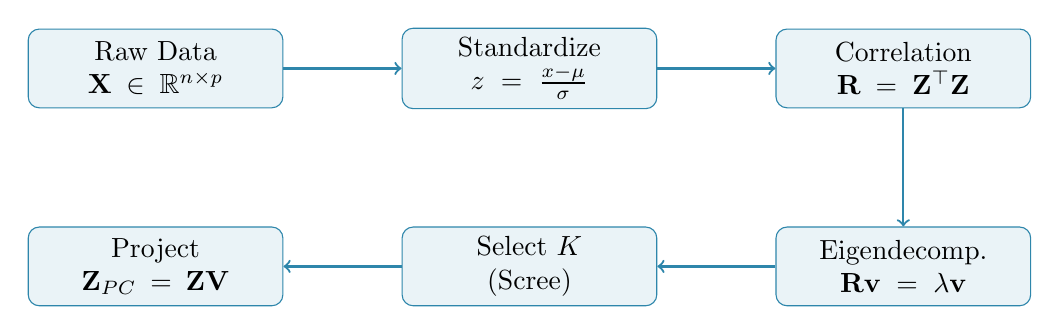
\begin{tikzpicture}[
            node distance=1.5cm,
            box/.style={rectangle, draw=primary, fill=primary!10, text width=3cm, align=center, minimum height=1cm, rounded corners},
            arrow/.style={->, thick, primary}
        ]
            \node[box] (data) {Raw Data\\$\mathbf{X} \in \mathbb{R}^{n \times p}$};
            \node[box, right=of data] (std) {Standardize\\$z = \frac{x-\mu}{\sigma}$};
            \node[box, right=of std] (corr) {Correlation\\$\mathbf{R} = \mathbf{Z}^\top\mathbf{Z}$};
            \node[box, below=of corr] (eig) {Eigendecomp.\\$\mathbf{R}\mathbf{v}=\lambda\mathbf{v}$};
            \node[box, left=of eig] (select) {Select $K$\\(Scree)};
            \node[box, left=of select] (project) {Project\\$\mathbf{Z}_{PC}=\mathbf{ZV}$};
            
            \draw[arrow] (data) -- (std);
            \draw[arrow] (std) -- (corr);
            \draw[arrow] (corr) -- (eig);
            \draw[arrow] (eig) -- (select);
            \draw[arrow] (select) -- (project);
        \end{tikzpicture}
    \end{center}
    
    \vspace{0.5cm}
    
    \textbf{Tools:} Python (NumPy, Pandas, Scikit-learn, Matplotlib)
\end{frame}

\begin{frame}{Future Directions}
    \begin{itemize}
        \item \textbf{Non-linear extensions:}
        \begin{itemize}
            \item Kernel PCA for non-linear relationships
            \item t-SNE/UMAP for visualization
        \end{itemize}
        
        \vspace{0.3cm}
        
        \item \textbf{Confirmatory analysis:}
        \begin{itemize}
            \item Factor Analysis with rotation
            \item Structural Equation Modeling
        \end{itemize}
        
        \vspace{0.3cm}
        
        \item \textbf{Temporal analysis:}
        \begin{itemize}
            \item Dynamic PCA for trend detection
            \item Time series decomposition
        \end{itemize}
    \end{itemize}
\end{frame}

\begin{frame}{}
    \begin{center}
        \Huge\textcolor{primary}{\textbf{Thank You!}}
        
        \vspace{1cm}
        
        \Large Questions?
        
        \vspace{1cm}
        
        \normalsize
        ST2DA-I2 | 2025-2026
    \end{center}
\end{frame}

%==============================================================================
% Backup Slides
%==============================================================================
\appendix

\begin{frame}{Backup: Mathematical Proof}
    \begin{block}{Proof: Variance = Eigenvalue}
        For principal component $\mathbf{z}_k = \mathbf{Z}\mathbf{v}_k$:
        \begin{align*}
            \text{Var}(\mathbf{z}_k) &= \frac{1}{n-1}\mathbf{z}_k^\top\mathbf{z}_k = \frac{1}{n-1}(\mathbf{Zv}_k)^\top(\mathbf{Zv}_k)\\
            &= \frac{1}{n-1}\mathbf{v}_k^\top\mathbf{Z}^\top\mathbf{Z}\mathbf{v}_k = \mathbf{v}_k^\top\mathbf{R}\mathbf{v}_k\\
            &= \mathbf{v}_k^\top(\lambda_k\mathbf{v}_k) = \lambda_k\underbrace{\mathbf{v}_k^\top\mathbf{v}_k}_{=1} = \lambda_k \quad \square
        \end{align*}
    \end{block}
\end{frame}

\begin{frame}{Backup: Complete Eigenvalue Table}
    \begin{center}
        \small
        \begin{tabular}{cccc}
            \toprule
            \textbf{PC} & $\boldsymbol{\lambda}$ & \textbf{Var.\%} & \textbf{Cum.\%} \\
            \midrule
            1 & 1.1147 & 7.43 & 7.43 \\
            2 & 1.0894 & 7.26 & 14.69 \\
            3 & 1.0799 & 7.20 & 21.89 \\
            4 & 1.0596 & 7.06 & 28.95 \\
            5 & 1.0448 & 6.97 & 35.92 \\
            6 & 1.0283 & 6.86 & 42.78 \\
            7 & 1.0107 & 6.74 & 49.52 \\
            8 & 0.9988 & 6.66 & 56.18 \\
            \midrule
            9 & 0.9834 & 6.56 & 62.74 \\
            10 & 0.9721 & 6.48 & 69.22 \\
            11 & 0.9602 & 6.40 & 75.62 \\
            12-15 & ... & ... & 100.00 \\
            \bottomrule
        \end{tabular}
    \end{center}
\end{frame}

\begin{frame}{Backup: References}
    \small
    \begin{enumerate}
        \item Jolliffe, I. T., \& Cadima, J. (2016). Principal component analysis: a review and recent developments. \textit{Phil. Trans. R. Soc. A}, 374(2065).
        
        \item Abdi, H., \& Williams, L. J. (2010). Principal component analysis. \textit{WIREs Comp. Stats.}, 2(4), 433-459.
        
        \item Pearson, K. (1901). On lines and planes of closest fit. \textit{Phil. Mag.}, 2(11), 559-572.
        
        \item Hotelling, H. (1933). Analysis of a complex of statistical variables. \textit{J. Ed. Psych.}, 24(6), 417-441.
        
        \item Kaiser, H. F. (1960). The application of electronic computers to factor analysis. \textit{Ed. \& Psych. Meas.}, 20(1), 141-151.
    \end{enumerate}
\end{frame}

\end{document}

